\chapter{Logical Viewpoint} \label{chp:logical-viewpoint-template}
	\begin{comment}
		The purpose of the Logical viewpoint is to elaborate existing and designed types and their implementations
		as classes and interfaces with their structural static relationships. This viewpoint also uses examples of
		instances of types in outlining design ideas.
	\end{comment}
	
	\section{Design concerns} \label{s:logical-viewpoint-template:design-concerns}
		\begin{comment}
			The Logical viewpoint is used to address the development and reuse of adequate abstractions and their
			implementations. For any implementation platform, a set of types is readily available for the domain
			abstractions of interest in a design subject, and a number of new types is to be designed, some of which
			may be considered for reuse. The main concern is the proper choice of abstractions and their expression in
			terms of existing types (some of which may had been specific to the design subject).
		\end{comment}
		The logical viewpoint is used to address the development and reuse of adequate abstractions and their implementations.
	\section{Design elements} \label{s:logical-viewpoint-template:design-elements}
		\begin{comment}
			Design entities: class, interface, power type, data type, object, attribute, method, association class, template,
			and namespace.
			
			Design relationships: association, generalization, dependency, realization, implementation, instance of,
			composition, and aggregation.
			
			Design attributes: name, role name, visibility, cardinality, type, stereotype, redefinition, tagged value,
			parameter, and navigation efficiency.
			
			Design constraints: value constraints, relationships exclusivity constraints, navigability, generalization sets,
			multiplicity, derivation, changeability, initial value, qualifier, ordering, static, pre-condition, post-condition,
			and generalization set constraints.
		\end{comment}
		
		\begin{design-element}{Sparse matrix formats}{Class Hierarchy}
			Diagram \ref{fig:sparse-matrices} presents all sparse matrix formats supported by \emph{Computational Library}. Distinguishing: \gls{CRS}, \gls{ELL} and \gls{MM}. All of those matrices are implemented as \emph{C++} templates, which allows user to specify the type of matrix values. This approach allows to extend existing classes to complex types.
			\begin{figure}[!hp]
				\centering
				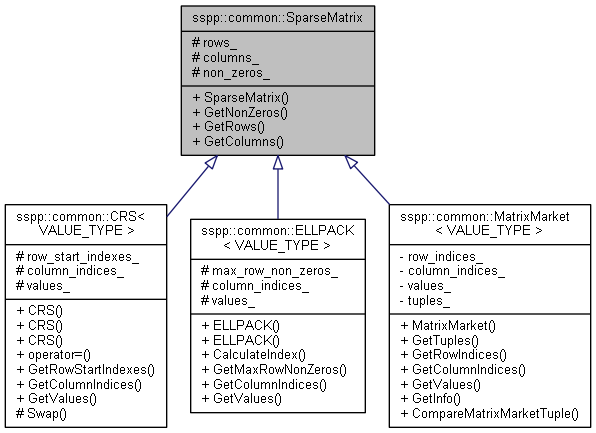
\includegraphics[scale=0.6]{others/img/sparse}
				\caption{Sparse matrix hierarchy classes.}
				\label{fig:sparse-matrices}
			\end{figure}
		\end{design-element}
	
		\begin{design-element}{\glsdesc{MM} Reader}{Collaboration}
			Diagram \ref{fig:mm-reader} presents function calls according to supported storage types and data types. As it is visualized reading \gls{MM} format is a two steps process. 
			\begin{figure}[!hp]
				\centering
				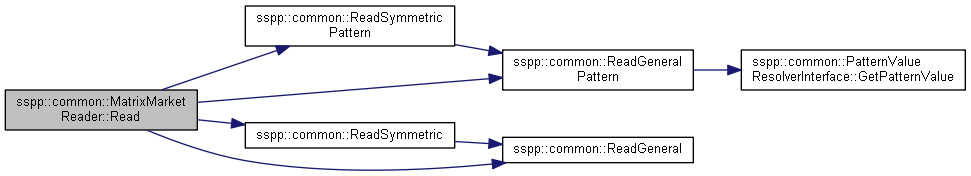
\includegraphics[width=\textwidth]{others/img/matrix-market-reader}
				\caption{\glsdesc{MM} format collaboration diagram.}
				\label{fig:mm-reader}
			\end{figure}
		\end{design-element}
	
		\begin{design-element}{\glsdesc{CRS} Transformer}{Collaboration}
			Diagram \ref{fig:crs-transformer} describes all the included classes and routines during transformation from \gls{MM} to \gls{CRS} formats.
			\begin{figure}[!hp]
				\centering
				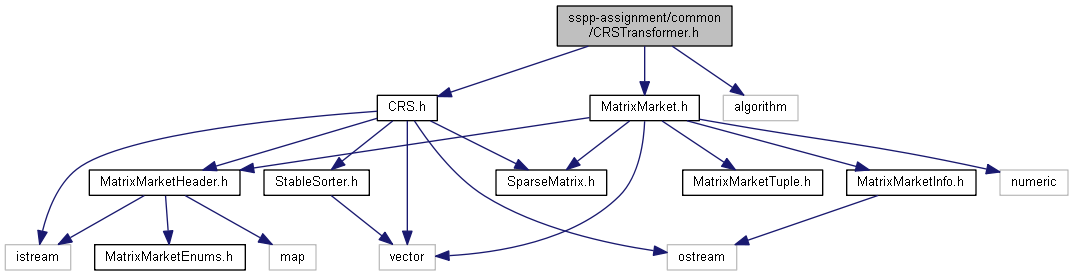
\includegraphics[width=\textwidth]{others/img/crs-transformer}
				\caption{\gls{CRS} Transformer collaboration diagram.}
				\label{fig:crs-transformer}
			\end{figure}
		\end{design-element}
		\clearpage
		\begin{design-element}{\glsdesc{ELL} Transformer}{Collaboration}
			Diagram \ref{fig:ell-transformer} describes all the included classes and routines during transformation from \gls{MM} to \gls{ELL} formats.
			\begin{figure}[!hp]
				\centering
				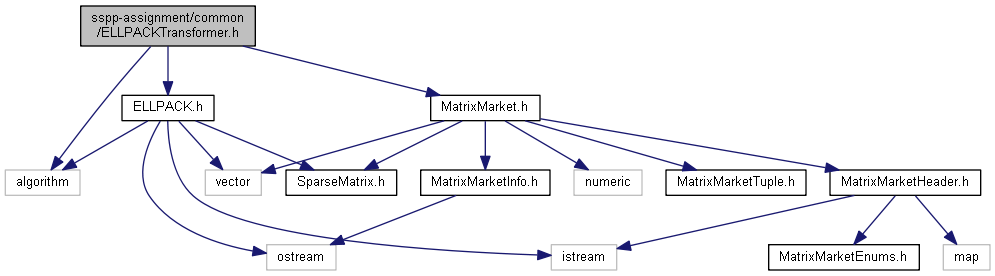
\includegraphics[width=\textwidth]{others/img/ellpack-transformer}
				\caption{\gls{ELL} Transformer collaboration diagram.}
				\label{fig:ell-transformer}
			\end{figure}
		\end{design-element}
	
		\begin{design-element}{Abstract \glsdesc{CRS} Solver}{Class hierarchy}
			Diagram \ref{fig:crs-solver} presents Abstract \gls{CRS} Solver class which is written using \emph{C++} templates for providing high extendability of library. We can distinguish tree different implementations for serial, \gls{cuda} and \gls{openmp} frameworks. Last one contains additional function to tune number of threads. 
			\begin{figure}[!hp]
				\centering
				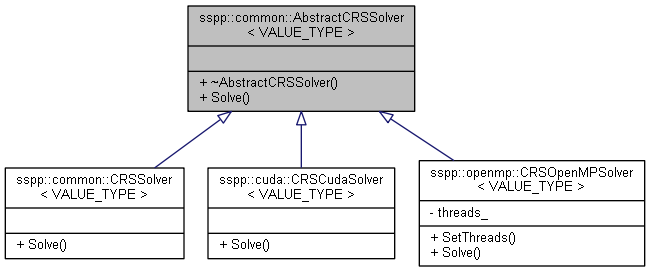
\includegraphics[scale=0.6]{others/img/abstract-crs-solver}
				\caption{Abstract \glsdesc{CRS} Solver class diagram.}
				\label{fig:crs-solver}
			\end{figure}
		\end{design-element}
		\clearpage
		\begin{design-element}{Abstract \glsdesc{ELL} Solver}{Class hierarchy}
				Diagram \ref{fig:ell-solver} presents Abstract \gls{ELL} Solver class which is written using \emph{C++} templates for providing high extendability of library. We can distinguish tree different implementations for serial, \gls{cuda} and \gls{openmp} frameworks. Last one contains additional function to tune number of threads. 
			\begin{figure}[!hp]
				\centering
				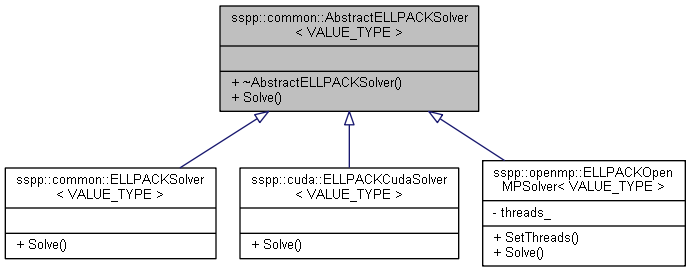
\includegraphics[scale=0.6]{others/img/abstract-elpack-solver}
				\caption{Abstract \glsdesc{ELL} Solver class diagram.}
				\label{fig:ell-solver}
			\end{figure}
		\end{design-element}
	
		\begin{design-element}{Abstract Stopwatch}{Collaboration}
			Abstract stopwatch presented in Diagram \ref{fig:abstract-stopwatch} is implemented in tree different ways depending on used framework. As we can see \texttt{ChronoStopwatch} is used for serial code, \texttt{OpenMPStopwatch} is used in \gls{openmp} module and the last \texttt{CUDAStopwatch} is used in \gls{cuda} module.
			\begin{figure}[!hp]
				\centering
				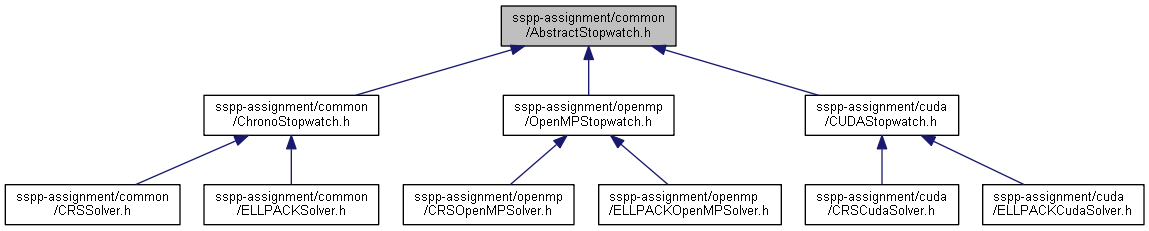
\includegraphics[width=\textwidth]{others/img/abstract-stopwatch-calls}
				\caption{Abstract stopwatch routines.}
				\label{fig:abstract-stopwatch}
			\end{figure}
		\end{design-element}
%	\section{Example languages} \label{s:logical-viewpoint-template:example-languages}
		\begin{comment}
			UML class diagrams and UML object diagrams (showing objects as instances of their respective classes)
			(OMG [B28]). Lattices of types and references to implemented types are commonly used as supplementary
			information.
		\end{comment}